\documentclass{article}
\usepackage{geometry}
\usepackage{float}
\usepackage[T1]{fontenc}
\usepackage[polish]{babel}
\usepackage[utf8]{inputenc}
\usepackage{graphicx}
\graphicspath{ {./images/} }

\geometry{
 a4paper,
 total={170mm,257mm},
 left=20mm,
 top=20mm,
}

\title{Analiza i przetwarzanie dźwięku - Projekt 3}
\date{\today}
\author{Mateusz Śliwakowski}

\begin{document}
  \pagenumbering{gobble}
  \maketitle
  \pagenumbering{arabic}
  
\section{Treść zadania}
Celem zadania było zaimplementowanie programu, który wczytuje plik audio, a następnie przeprowadza jego analizę w dziedzinie częstotliwości na poziomie ramki. Należało zbadać cztery parametry - \textit{Volume, Frequency Centroid, Effective Bandwidth} oraz \textit{Band Energy}.

\section{Opis aplikacji}

Aplikację zdecydowałem się wykonać w języku \textit{C\#}, w środowisku \textit{WinForms}. Jako, że w zadaniu można było wykorzystać znaczną część implementacji z projektu 2 zdecydowałem, że zamiast tworzyć nowe rozwiązanie, projekt zrealizuję poprzez rozwój poprzedniego. Prace rozpocząłęm od dodania zakładek z nowymi parametrami.

\begin{figure}[H]
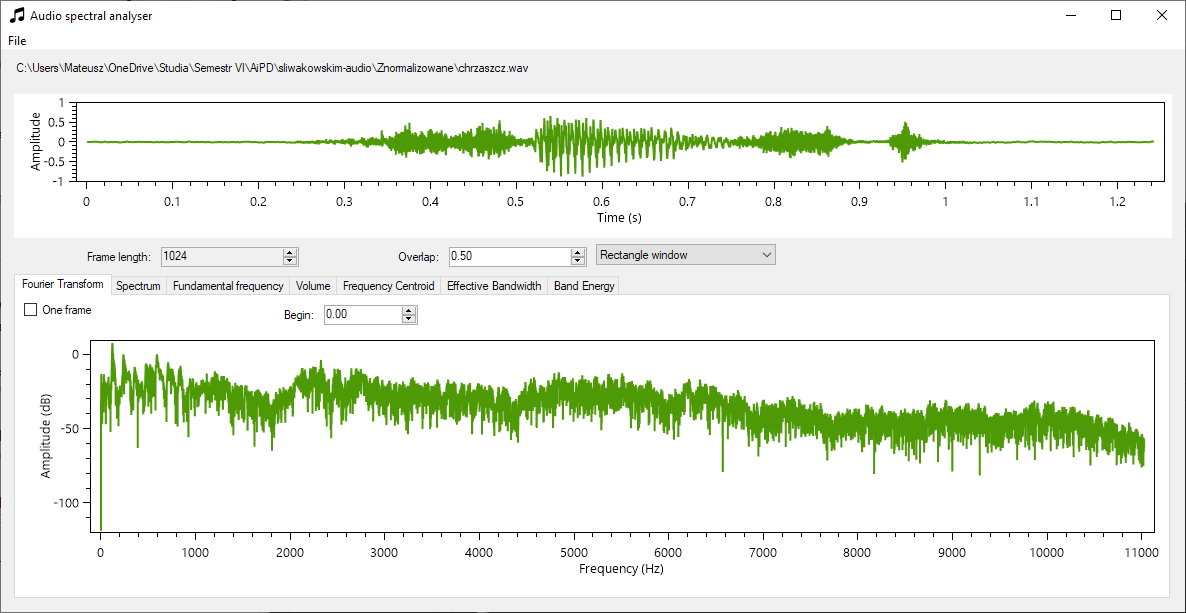
\includegraphics[width=6in]{scr1.png}
\centering
\caption{Interfejs użytkownika}
\end{figure}

\noindent Użyte technologie pozostały bez zmian. Do obsługi plików audio użyłem biblioteki \textit{NAudio}, do rysowania wykresów \textit{OxyPlot}, a do obliczania FFT \textit{MathNet Numerics}.

\section{Zaimplementowane metody}
\subsection{Wstęp}
Wszystkie zaimplementowane metody opierały się na analizowaniu sygnału audio w dziedzinie częstotliwości na poziomie ramki. Wejściowy sygnał był dzielony na ramki o zadanej długości (zachodziły one na siebie zgodnie z wartością parametru \textit{overlap}).

\subsection{Volume}
Głośność w tym opracowaniu wyznaczana była w inny sposób, niż w projekcie pierwszym. Dla danej ramki określona była następującym wzorem:
$$Vol(n) = \frac{1}{N}\sum^{N-1}_{k=0}S_n^2(k),$$
gdzie $S_n$ to wynik transformaty Fouriera dla ramki o indeksie n, a $N$ to długość ramki.

\subsection{Frequency Centroid}
Kolejnym badanym parametrem był \textit{Frequency Centroid}. Określa on gdzie zlokalizowany jest środek ciężkości dla spektogramu. Dla odbiorcy odpowiada wrażeniu jasności dźwięku. Wyraża się wzorem:
$$FC(n)=\frac{\int_{0}^{\infty} \omega S_n(\omega)d\omega}{\int_0^\infty S_n(\omega)d\omega},$$
gdzie $\omega$ to częstotliwość. Ze względu na fakt dyskretyzacji danych, całka w implementacji została zamieniona na sumę.

\subsection{Effective Bandwidth}
Używając obliczonego \textit{Frequency Centroid} można policzyć parametr bezpośrednio z nim związany, czyli \textit{Effective Bandwidth}. Określa on odchylenie standardowe częstosliwości, przez co dobrze określa szerokość pasma. Wyraża się wzorem:
$$BW^2(n)=\frac{\int_0^\infty(\omega-FC(n))^2S_n^2(\omega)d\omega}{\int_0^\infty(\omega)d\omega}.$$
Również w tym przypadku, konieczne było zamienienie całki na sumę w implementacji.

\subsection{Band Energy}
Ostatnim parametrem było \textit{Band Energy}, obliczane w przedziale częstotliwości od $f_0$ do $f_1$. Określa ono energię w spektrum sygnału i określony jest wzorem:
$$BE_{[f_0,f_1]}(t)=\frac{\int_{f_0}^{f_1}S_t^2(f)df}{\int w(\tau)d\tau},$$
gdzie $w$ jest oknem analizy.

\section{Wyniki działania programu}

\subsection{Volume}
Obliczanie głośności za pomocą analizy spektralnej dało zadowalające wyniki. Porównując rezultaty do tych, otrzymanych za pomocą analizy amplitudy sygnału otrzymujemy wykres o podobnej charakterystyce, lecz pozbawiony szumów. Warto jednak zauważyć, że ten typ wyznaczania głośności jest bardziej skomplikowany obiczeniowo, ponieważ dla każdej ramki wymaga liczenia FFT.

\begin{figure}[H]
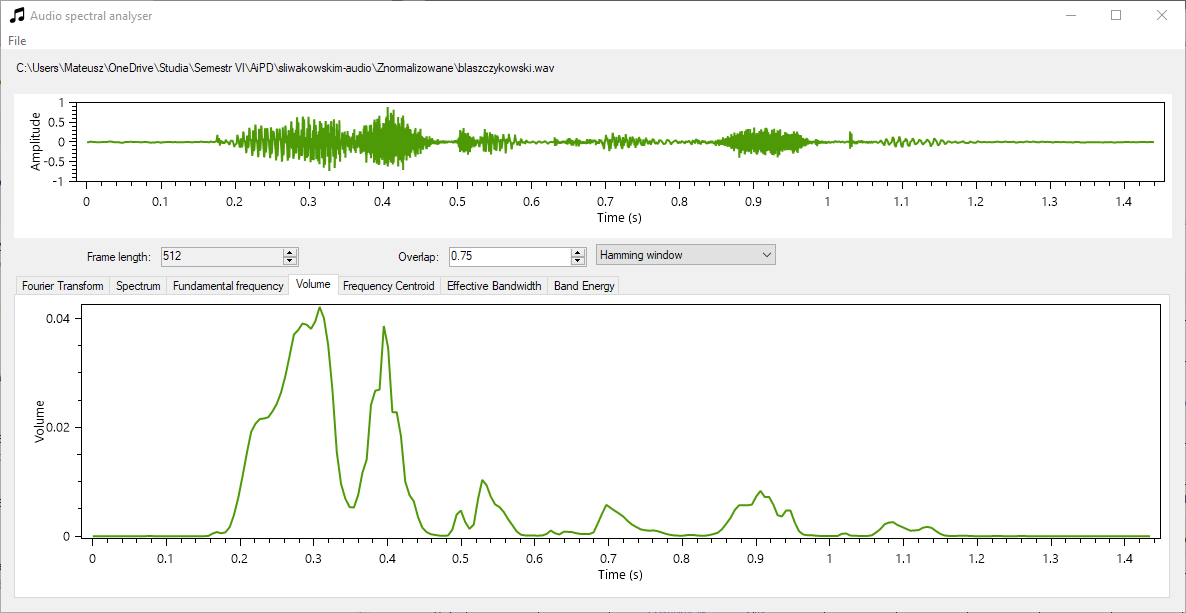
\includegraphics[width=6in]{scr2.png}
\centering
\caption{Głośność nagrania 'blaszczykowski.wav', analiza spektralna}
\end{figure}

\begin{figure}[H]
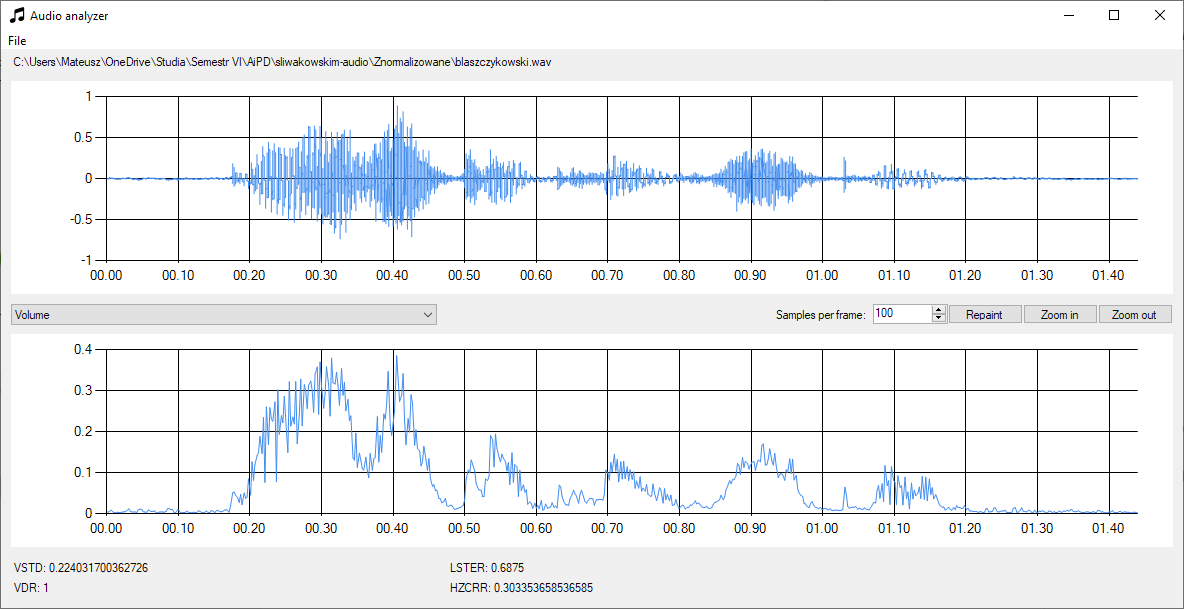
\includegraphics[width=6in]{scr3.png}
\centering
\caption{Głośność nagrania 'blaszczykowski.wav', analiza amplitudowa}
\end{figure}

\subsection{Frequency Centroid}
Parametr Frequency Centroid sprawdza się w rozróżnianiu mowy od muzyki. Dla samej mowy, powinniśmy otrzymać wartości w zakresie 125-8000Hz. 

\begin{figure}[H]
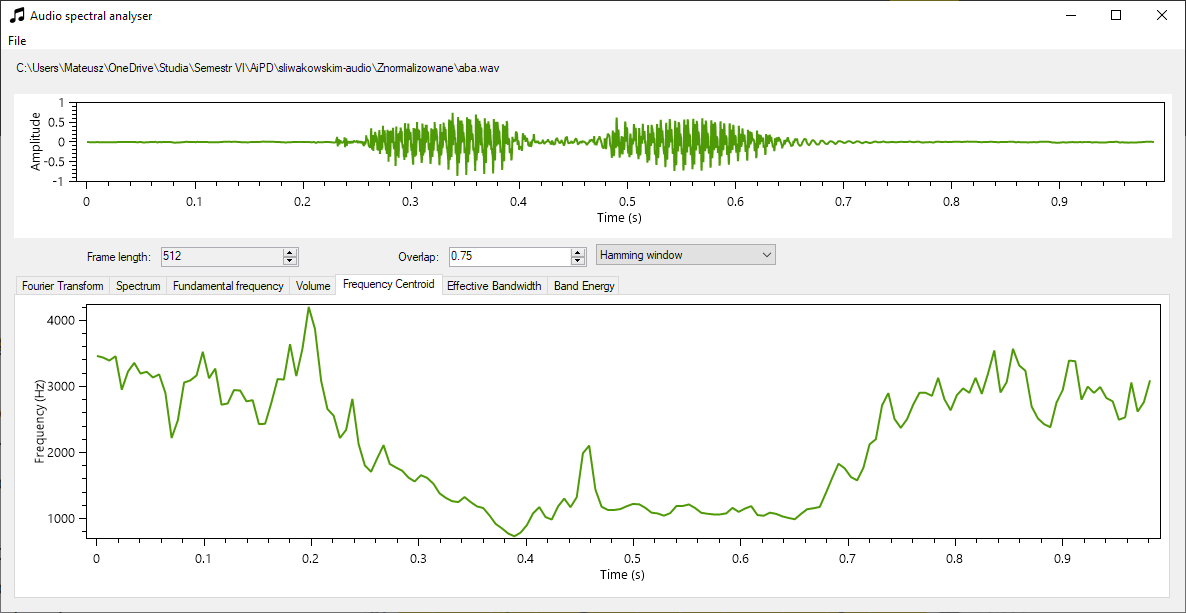
\includegraphics[width=6in]{scr4.png}
\centering
\caption{Frequency Centroid nagrania 'aba.wav'}
\end{figure}

\noindent Faktycznie, dla słowa 'aba' otrzymujemy wartości zbliżone do oczekiwanych. Częstotliwość samogłoski 'a' powinna zawierać się w zakresie 500-1000Hz. Na powyższym zdjęciu widzimy, że jest ona bardzo zbliżona do wzorcowego rezultatu. Dla muzyki o agresywnej charakterystyce otrzymujemy wartości zdecydowanie wyższe:

\begin{figure}[H]
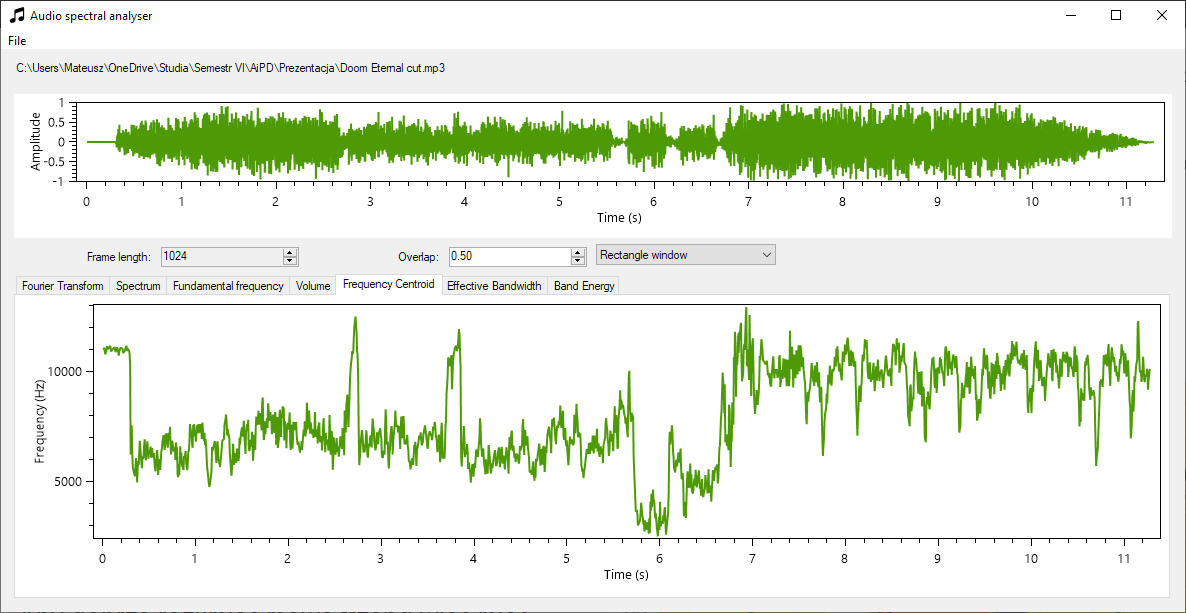
\includegraphics[width=6in]{scr5.png}
\centering
\caption{Frequency Centroid nagrania 'Doom Eternal cut.wav'}
\end{figure}

\noindent Ciekway rezultat uzyskujemy dla nagrania o stałej częstotliwości 400Hz. Otrzymujemy wykres o bardzo regularnej, lecz nieoczekiwanej charakterystyce.

\begin{figure}[H]
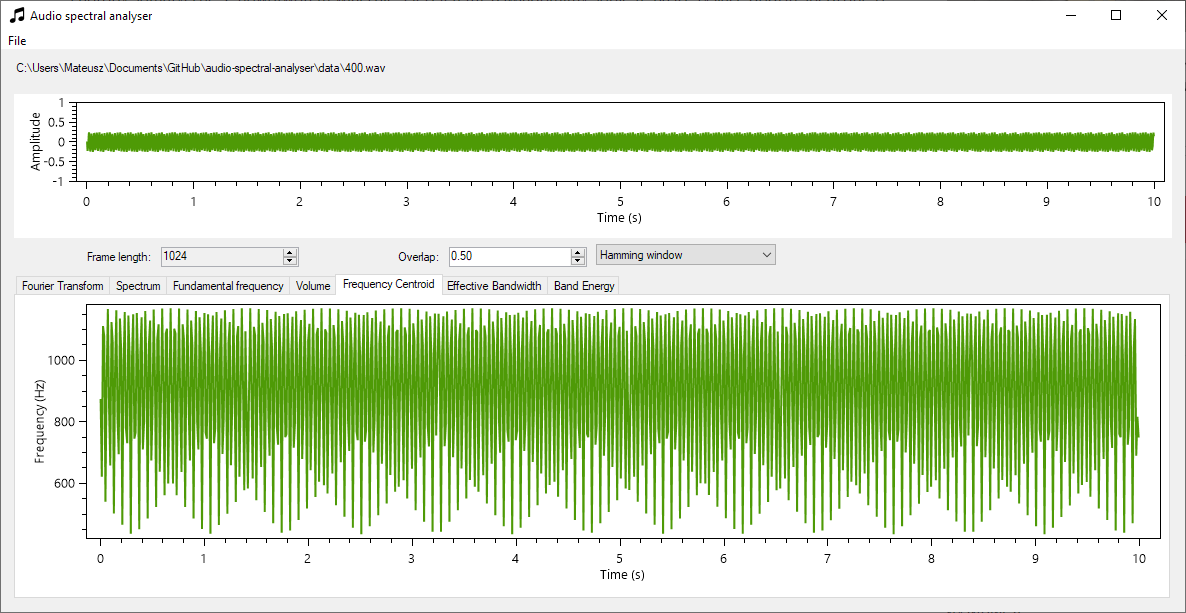
\includegraphics[width=6in]{scr6.png}
\centering
\caption{Frequency Centroid nagrania '400.wav'}
\end{figure}

\noindent Dobierając odpowiednią ramkę oraz długość ramki jesteśmy w stanie uzyskać centroid o wartości 400Hz. Jest to spowodowane charakterystycznym wpływem okna van Hanna na ten parametr.

\begin{figure}[H]
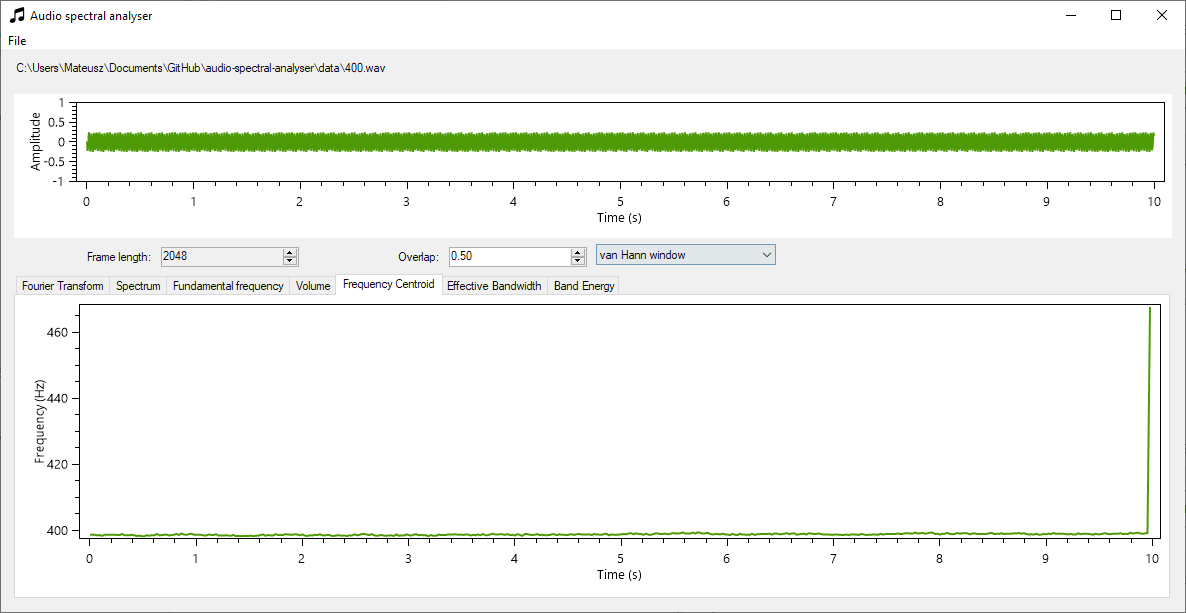
\includegraphics[width=6in]{scr7.png}
\centering
\caption{Frequency Centroid nagrania '400.wav', okno van Hanna}
\end{figure}

\subsection{Effective Bandwdith}
Parametr \textit{Effective Bandwidth} jest bezpośrednio skorelowany z parametrem \textit{Frequency Centroid}. Oczekujemy, że dla mowy będzie przyjmował niższe wartości, niż dla muzyki.

\begin{figure}[H]
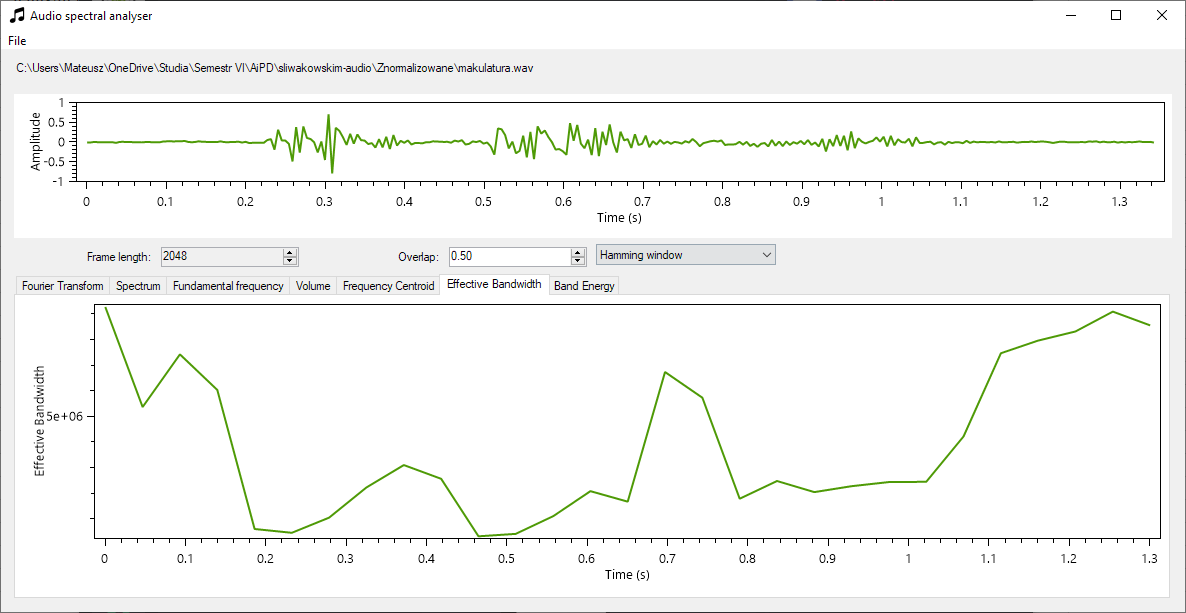
\includegraphics[width=6in]{scr8.png}
\centering
\caption{Effective Bandwidth nagrania 'makulatura.wav'}
\end{figure}

\begin{figure}[H]
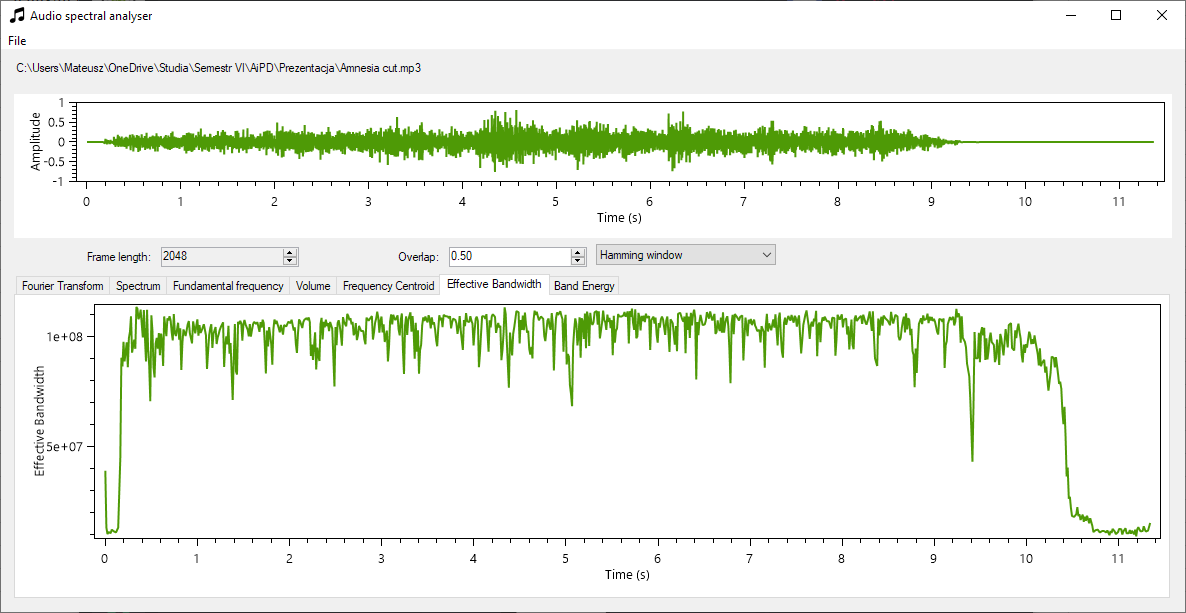
\includegraphics[width=6in]{scr9.png}
\centering
\caption{Effective Bandwidth nagrania 'Amnesia cut.wav'}
\end{figure}

\noindent Wyniki spełniają oczekiwania - wartość \textit{Effective Bandwidth} dla muzyki jest zdecydowanie wyższa.

\subsection{Band Energy}
Wartość tego parametru w pełnym zakresie częstotliwości może posłużyć nam do wykrywania ciszy. Daje bardziej wiarygodne rezultaty niż np. ZCR, który miał tendencje do oscylacji, przez co dla niektórych nagrań wyniki były dalekie od oczekiwań. Kiedy ograniczymy analizę do konkretnego zakresu częstotliwości, również i ten parametr może posłużyć do rozróżniania mowy od muzyki.

\begin{figure}[H]
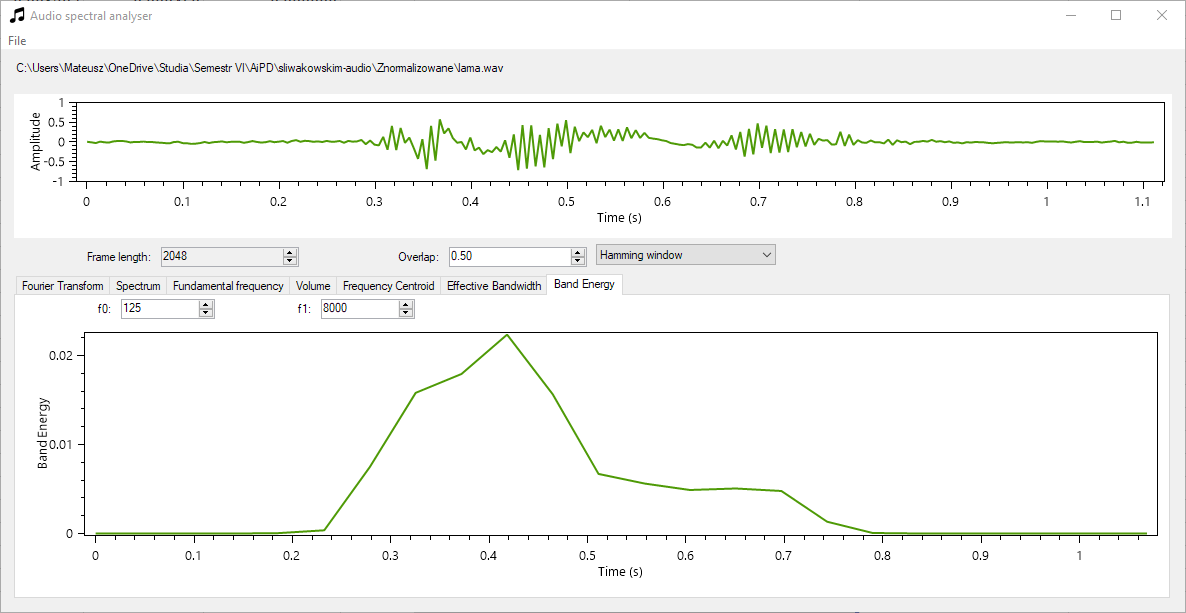
\includegraphics[width=6in]{scr10.png}
\centering
\caption{Band Energy nagrania 'lama.wav', zakres 125-8000Hz}
\end{figure}

\begin{figure}[H]
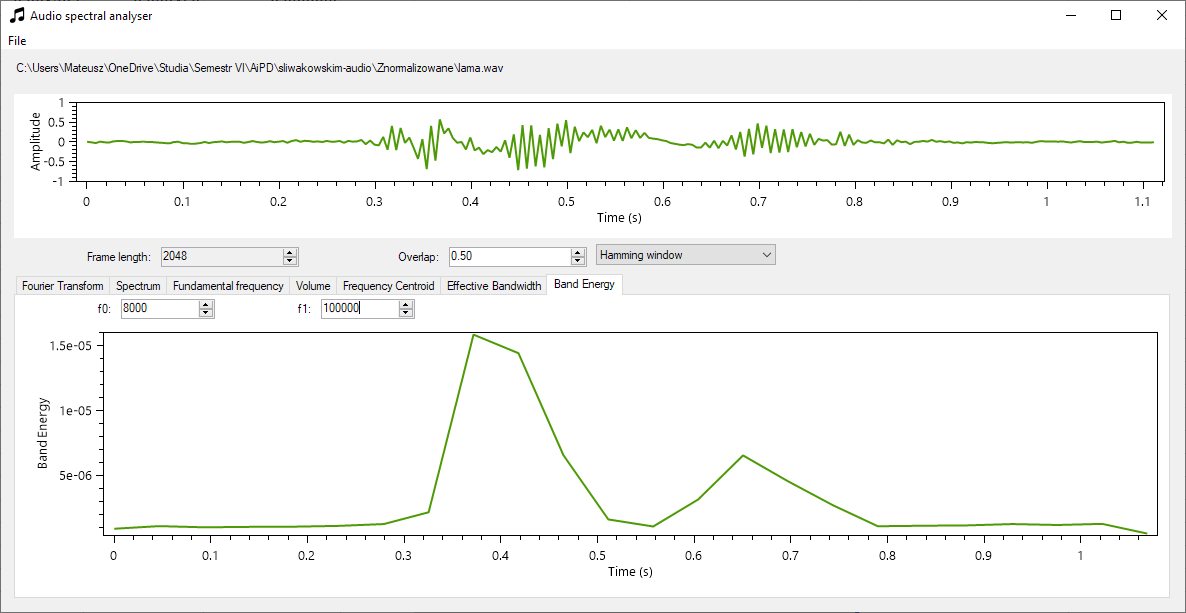
\includegraphics[width=6in]{scr11.png}
\centering
\caption{Band Energy nagrania 'lama.wav', zakres 8000-100000Hz}
\end{figure}

\begin{figure}[H]
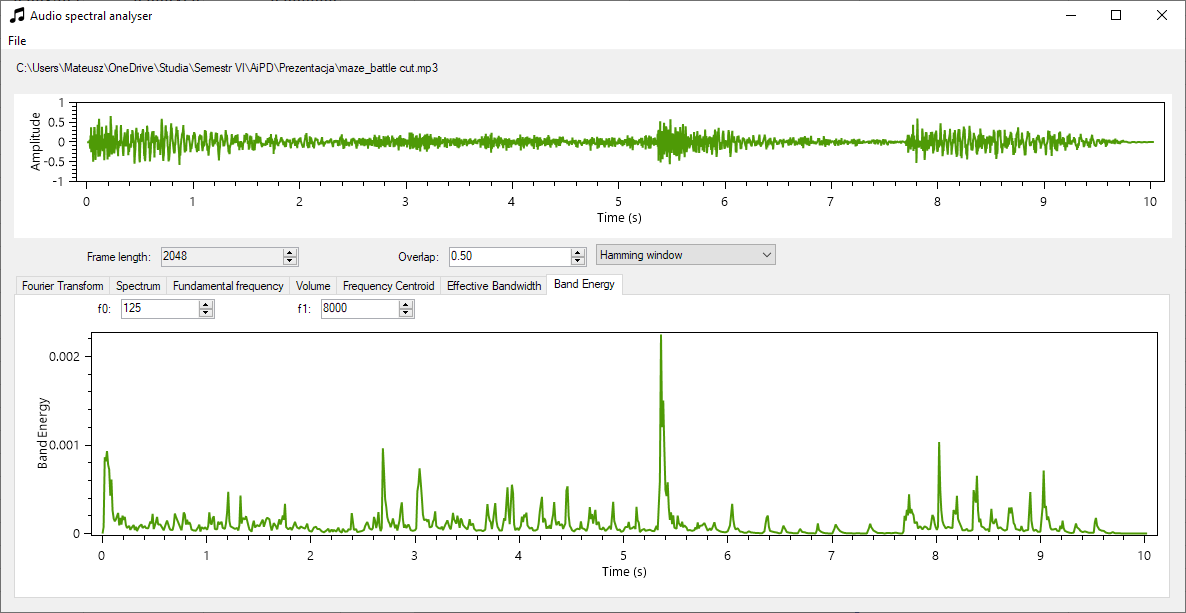
\includegraphics[width=6in]{scr12.png}
\centering
\caption{Band Energy nagrania 'maze battle cut.wav', zakres 125-8000Hz}
\end{figure}

\begin{figure}[H]
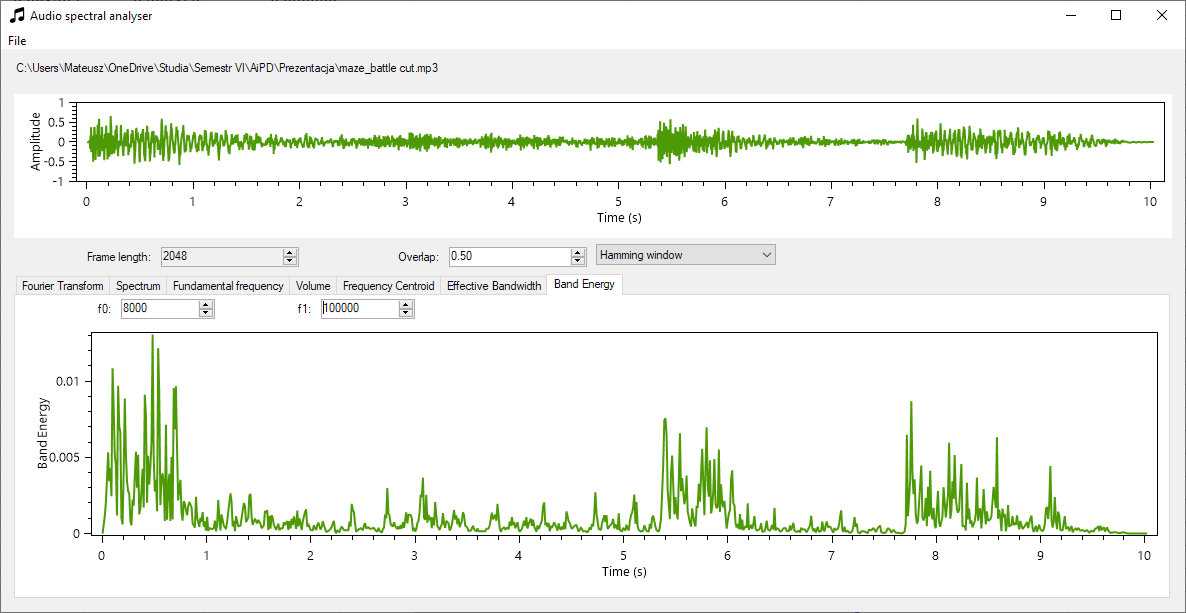
\includegraphics[width=6in]{scr13.png}
\centering
\caption{Band Energy nagrania 'maze battle cut.wav', zakres 8000-100000Hz}
\end{figure}

\section{Wnioski}
\subsection{Implementacja}
Posiadając podłoże do pracy w postaci projektu drugiego, implementacja przebiegła szybko i sprawnie. Można było się oprzeć na kluczowych funkcjonalnościach takich jak podział sygnału na ramki, obliczanie transformaty Fouriera, czy rysowanie wykresów. Trudność sprawić mogło dostosowanie wzorów z całkami do obliczeń dyskretnych, lecz nie były one na tyle skomplikowane, aby okazało się to dużą przeszkodą.

\subsection{Wyniki analizy audio}
Analiza audio na poziomie ramki w dziedzinie częstotliwości dostarcza ciekawych i przydatnych parametrów. Otrzymujemy oczekiwaną charakterystykę głośności, nieco lepszą niż w przypadku analizy amplitudy. Parametry \textit{Frequency Centroid} oraz \textit{Effective Bandwidth} mogą posłużyć do rozróżniania muzyki oraz mowy. Wartość \textit{Band Energy} mogłaby zaś posłużyć jako wskaźnik pomocny przy wykrywaniu ciszy.

\begin{figure}[b]
\centering
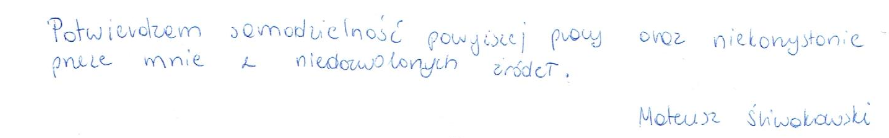
\includegraphics[width=5in]{bottom.png}
\end{figure}

\end{document}

